\begin{frame}
\frametitle{Prym varieties}


\begin{itemize}
	\item Start with an étale double cover \alert{$\widetilde C \xrightarrow{\pi} C$}.
	\pause
	\item Apply the Jacobian functor $J(-)$ to get a morphism:
	\begin{align*}
	\Nm:J(\widetilde C) &\to J(C) \\
	\OO_{\widetilde C}(\widetilde D) &\mapsto \OO_C(\pi_\ast \widetilde D).
	\end{align*}
	\pause

	\item Then:
	\alert{
	\[
	\Prym(\widetilde C, C) := \left(\ker \Nm \right)_0.
	\]
	}
\end{itemize}

\end{frame}


\begin{frame}
\frametitle{First properties of Pryms}

\begin{itemize}
	\item Every double cover comes with an involution $\sigma:  \widetilde C \circlearrowleft$ exchanging sheets.
\end{itemize}


\begin{proposition}
\[
(\ker Nm)_0 = \mathrm{Im}(1-\sigma).
\]
\end{proposition}
\begin{proof}["Proof"]
One way is okay. Suppose $D= \sum a_i P_i - \sum a_i \sigma{P_i}$ is in the image. Then
\[
\Nm(D) = \sum a_i P_i - \sum a_i P_i = 0.
\]
\end{proof}
\end{frame}

\begin{frame}
\frametitle{The induced polarization}

The induced polarization comes from \alert{$i^\ast \Theta$}, where $i:\Prym(\widetilde C, \C) \to J(\widetilde C)$ is the inclusion.

\begin{theorem}
The induced polarization on $P$ is twice a principal polarization.
\end{theorem}
\pause
\begin{remark}
In the complex setting, polarizations correspond to Hermitian forms on $\C^n$. It is principal if the Hermitian form can be written as 
\[
\begin{pmatrix}
0 & I \\
-I &0
\end{pmatrix}
\]
in the standard basis.
\end{remark}
\end{frame}

\begin{frame}
\frametitle{Set-up}

\begin{itemize}
	\item Recall the description of $J(\widetilde C)$ as $H^0(\widetilde C, \omega_{\widetilde C})^\ast/H_1(\widetilde C, \Z)$.
	\item We can identify
	\alert{
	\[
	\Prym(\widetilde C, C) = \left(H^0(\widetilde C, \omega_{\widetilde C})^\ast\right)^- /{H_1(\widetilde C, \Z)}^-,
	\]
	}
	where the $(-)^-$, denotes the $-1$-eigenspaces.
\end{itemize}



\end{frame}


    \setbeamertemplate{navigation symbols}{}
    \begin{frame}[plain]
        \begin{tikzpicture}[remember picture,overlay]
            \node[at=(current page.center)] {
                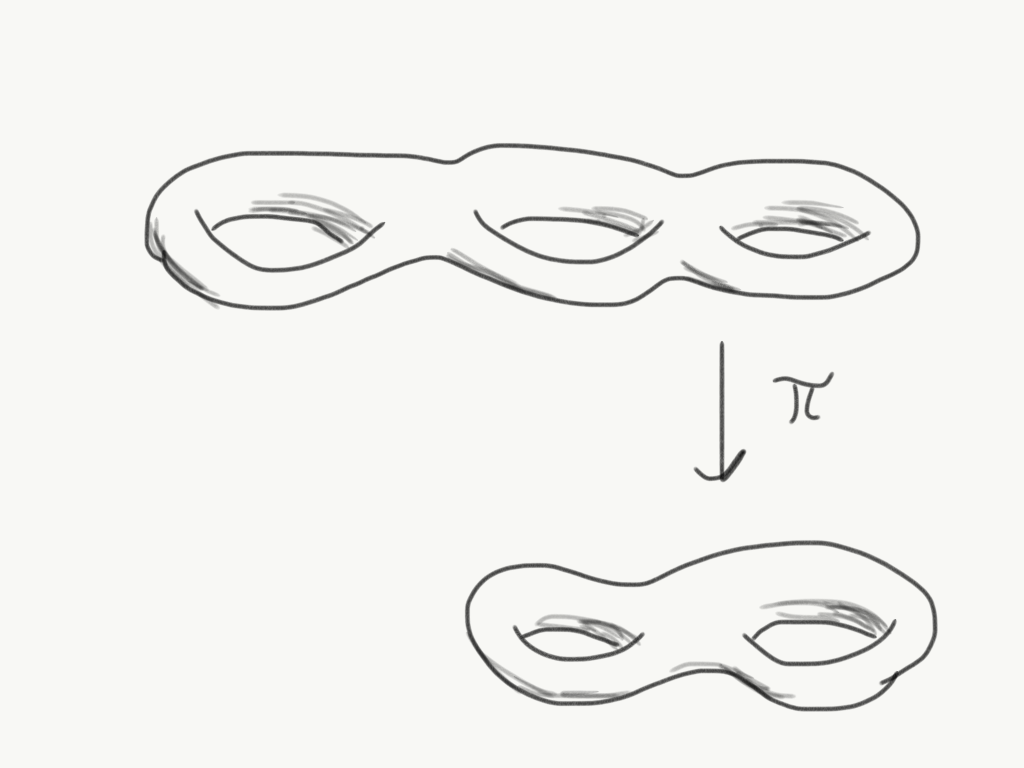
\includegraphics[width=\paperwidth]{sections/torus1}
            };
        \end{tikzpicture}
     \end{frame}

         \setbeamertemplate{navigation symbols}{}
    \begin{frame}[plain]
        \begin{tikzpicture}[remember picture,overlay]
            \node[at=(current page.center)] {
                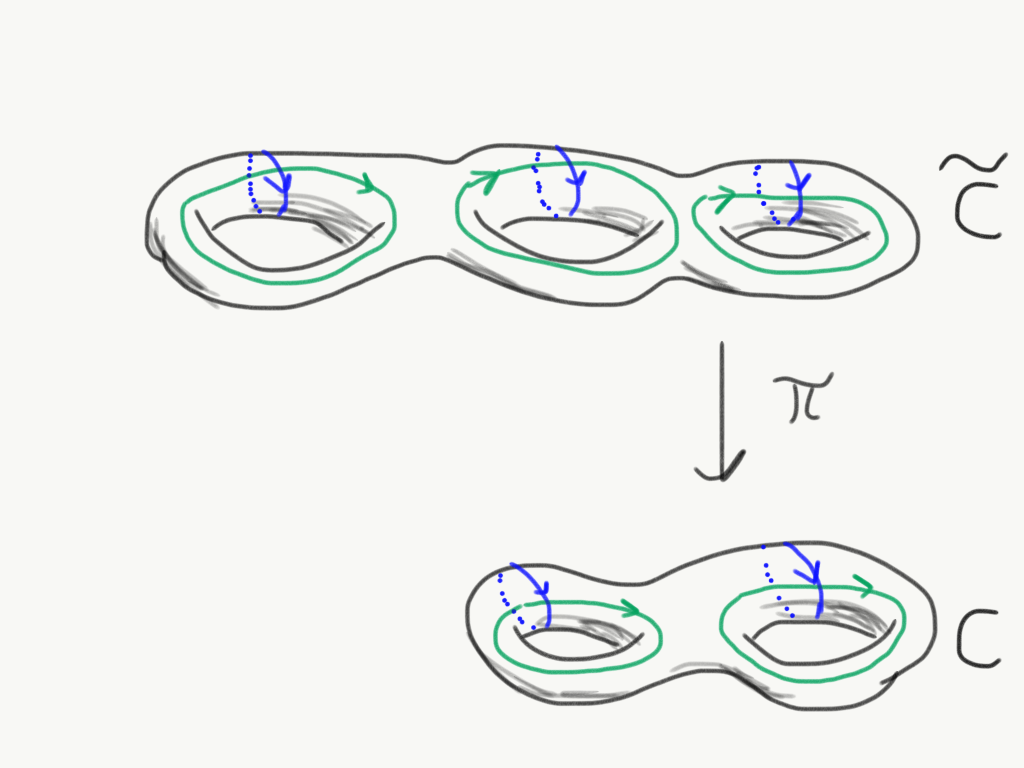
\includegraphics[width=\paperwidth]{sections/torus2}
            };
        \end{tikzpicture}
     \end{frame}


    \setbeamertemplate{navigation symbols}{}
    \begin{frame}[plain]
        \begin{tikzpicture}[remember picture,overlay]
            \node[at=(current page.center)] {
                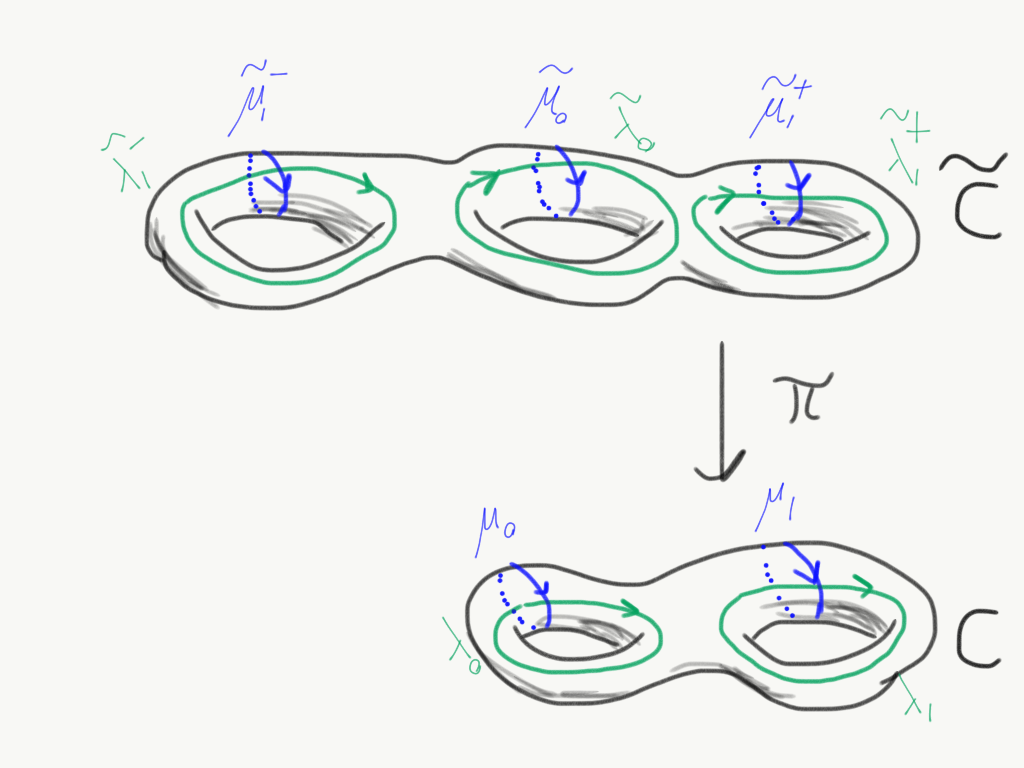
\includegraphics[width=\paperwidth]{sections/torus3}
            };
        \end{tikzpicture}
     \end{frame}


\begin{frame}

\begin{enumerate}
	\item Choose a symplectic basis $\lambda_0, \ldots, \lambda_g$, $\mu_0, \ldots, \mu_g$ of $H_1(C,\Z)$.
	\pause
	\item A degree $2$ covering is determined by a cycle $\mu_0$ in $H_1(C, \Z/2)$.
	\pause
	\item A symplectic basis for $H_1(\widetilde C, \Z)$ are the lifts $\widetilde{\mu^+}_i, \widetilde{\mu^-}_i$, $\widetilde{\lambda^-}_i, \widetilde{\lambda^+}_i$ and $\widetilde{\mu}_0, \widetilde{\lambda}_0$. (from this we see that $\widetilde C$ has genus $2g+1$ if $C$ has genus $g-1$)
	\pause
	\item A basis for the $(-1)$-eigenspace of $H_1(\widetilde C,\Z)$ is then
	\begin{align*}
	\alpha_i := \lambda_i^+ - \lambda_i^-, && \beta_i := \mu_i^+ - \mu_i^- && i=1,\ldots, g
	\end{align*}
	\pause
	\item The restriction of the Hermitian form is:
	\begin{align*}
	E(\alpha_i,\beta_j)= 2 \delta_{ij} && E(\alpha_i, \alpha_j) = E(\beta_i,\beta_j)=0,
	\end{align*}
	which means it is twice a principal polarization.
\end{enumerate}


\end{frame}